\documentclass[a4paper]{article}
\usepackage[pdftex]{graphicx}
\usepackage[utf8]{inputenc}
\usepackage{enumerate}
\usepackage{siunitx}
\sisetup{locale=DE} 
\usepackage{icomma}
\usepackage{amssymb}
\usepackage{tikz}
\usepackage{href-ul}
\hypersetup{
	colorlinks=true,
	linkcolor=blue,
	urlcolor=blue}
\usepackage{geometry}
\geometry{a4paper, top=15mm, left=15mm, right=15mm, bottom=15mm,
	headsep=10mm, footskip=12mm}

\begin{document}
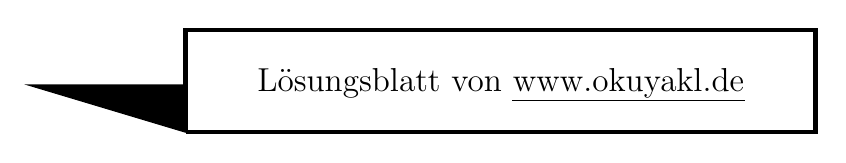
\begin{tikzpicture}(10,3)
	\draw[ultra thick](2,0) --(10,0) -- (10,1.3) --(2,1.3) -- (2,0);
	\draw[fill=black](2,0)-- (0,.6) -- (2,.6) -- (2,0);
	\node at (6,.6) {\large Lösungsblatt von \href{https://www.okuyakl.de}{www.okuyakl.de}};
\end{tikzpicture}
\vspace{0.5 cm}

\noindent{\bf Aufgabe 1. a)}\\
Die Zentripetalkraft muss gleich oder größer sein als die Gewichtskraft. Dann folgt für die Winkelgeschwindigkeit:
$$
\renewcommand{\arraystretch}{2}
\begin{array}{rcll}
m \omega^2 r &\ge& m g \\
\omega &\ge& \sqrt{g \over r}  & \stackrel{r=\SI{6,0}{\meter}}{\Longrightarrow} \quad \omega = \SI{1,27}{1 \over s}
\end{array}
$$
\vspace{0.5 cm}

\noindent{\bf Aufgabe 1. b)}\\
$$f = {\omega \over 2 \pi } = {1 \over 2 \pi } \cdot \sqrt{g \over r} \quad \stackrel{r=\SI{6,0}{\meter}}{\Longrightarrow} \quad f =  \SI{0,20}{\hertz}$$
\vspace{0.5 cm}

\noindent{\bf Aufgabe 1. c)}\\
$$ T = {1\over f} = 2\pi \cdot \sqrt{r \over g} \quad \stackrel{r=\SI{6,0}{\meter}}{\Longrightarrow} \quad T = \SI{4,9}{\second}$$
\vspace{0.5 cm}

\noindent{\bf Aufgabe 1. d)}\\
$$ v = \omega r = \sqrt{gr} \quad \stackrel{r=\SI{6,0}{\meter}}{\Longrightarrow} \quad v = \SI{7,7}{\meter\over\second}$$
\vspace{0.5 cm}

\noindent{\bf Aufgabe 2.}\\
Im Punkt A muss die Zentripetalkraft größer oder gleich sein wie die Gewichtskraft, also gilt für die Bahngeschwindigkeit in diesem Punkt:
$$v_A = \sqrt{gr}$$
Und damit für die kinetische Energie hier:
$$E_{kinA}={1 \over 2 } m\cdot g \cdot r$$
Im unteren Startpunkt ist die kinetische Energie höher, und zwar um den Betrag der potentiellen Energie:
$$E_{kinS}=E_{kinA}+E_{pot}={1 \over 2 } m g \cdot r +  m g\cdot 2r= 2,5 ~m g r $$
Dies setzen wir gleich mit der Spannenergie der Feder:
$$
\renewcommand{\arraystretch}{2}
\begin{array}{rcll}
E_{Sp}&=&{1\over 2} D s^2 = 2,5 ~mgr\\
s^2 &=& 5,0 {mgr \over D} \\
s &=& \sqrt{5,0 {mgr \over D}}  &= \SI{0,30}{\meter}
\end{array}
$$
\vspace{0.5 cm}

\newpage
\noindent{\bf Aufgabe 3. a)}\\
\noindent
\begin{minipage}{0.5\textwidth}
Für den Radfahrer gilt das Kräfterechteck, dass von der Zentrifugalkraft und der Gewichtskraft aufgespannt wird. Für den Winkel $\alpha$ gilt:
$$
\renewcommand{\arraystretch}{2}
\begin{array}{rcll}
\tan \alpha &=& { F_Z \over F_G}\\
\tan \alpha &=& {m v^2 \over m g r} \\
\tan \alpha &=& { v^2 \over  g r} \\
\tan \alpha &=& { ( \SI{6,0}{\meter\over \second})^2 \over  \SI{9,81}{\meter\over {\second^2}} \cdot \SI{30}{\meter}}\\
\tan \alpha &=& 0,122 \\
\alpha &=& \SI{7,0}{\degree}
\end{array}
$$
\end{minipage}
\hfill
\begin{minipage}{0.5\textwidth}
	\includegraphics[width=7 cm]{fara415}
\end{minipage}
\vspace{0.5 cm}

\noindent{\bf Aufgabe 3. b)}\\
Der Haftreibungskoeffizient $\mu$ entspricht dem maximalen Verhältnis von horizontaler zu vertikaler Kraft, was hier genau $\tan \alpha $ ist:
$$ \tan \alpha_{max} = 0,7 \quad \Rightarrow \quad \alpha_{max}= \SI{35}{\degree}$$
\vspace{0.5 cm}

\noindent{\bf Aufgabe 4.}\\
Wir setzen Haftreibungskraft gleich der Zentripetalkraft:
$$
\renewcommand{\arraystretch}{2}
\begin{array}{rclll}
F_R &=& F_Z \\
m \cdot {v^2 \over r} &=& \mu \cdot m g \\
 v &=& \sqrt{\mu \cdot  g r} &= \sqrt{0,80 \cdot \SI{9,81}{\meter\over {\second^2}} \cdot \SI{50}{\meter}} &=\SI{20}{\meter\over\second}
\end{array}
$$
\vspace{0.5 cm}

\noindent{\bf Aufgabe 5.}\\
Zur Berechnung wählen wir wie in Aufgabe 3. den Ansatz:
$$
\renewcommand{\arraystretch}{2}
\begin{array}{rcll}
\tan \alpha &=& { F_Z \over F_G}\\
\tan \alpha &=& { v^2 \over  g R} \\
v &=& \sqrt{\tan\alpha \cdot g R}
\end{array}
$$
Hier ist R der gesamte Radius:
$$R=r+l\cdot \sin\alpha = 3,0 + 3,5 \cdot \sin \SI{20}{\degree} = \SI{4,2}{\meter}$$
Wir setzen ein und erhalten für $v$:
$$\Rightarrow \quad v = \sqrt{\tan \SI{20}{\degree}\cdot \SI{9,81}{\meter \over {\second^2}} \cdot \SI{4,2}{\meter}}=\SI{3,9}{\meter\over\second}$$
Die Umlaufdauer T ist:
$$T ={2 \pi R \over v} = \SI{6,8}{\second}$$

\begin{center}
	\includegraphics[width=7 cm]{../../viecher/endcomic.pdf}
	
	Hier geht es zurück zum \href{https://www.okuyakl.de/phys/p10krbL415/aa415.pdf}{Aufgabenblatt}
\end{center}

\end{document}
